%!TEX root = ../thesis.tex

\section{目標方向}
本研究で用いた目標方向と, そのデータ形式である目標方向指令について述べる. 目標方向を\figref{Fig:direction}に示す. 経路と分岐路において「道なり」に走行(Go straight), 分岐路において「直進(Go straight)」, 「左折(Turn left)」, 「右折(Turn right)」の3つとする.

\begin{figure}[hbtp]
  \centering
 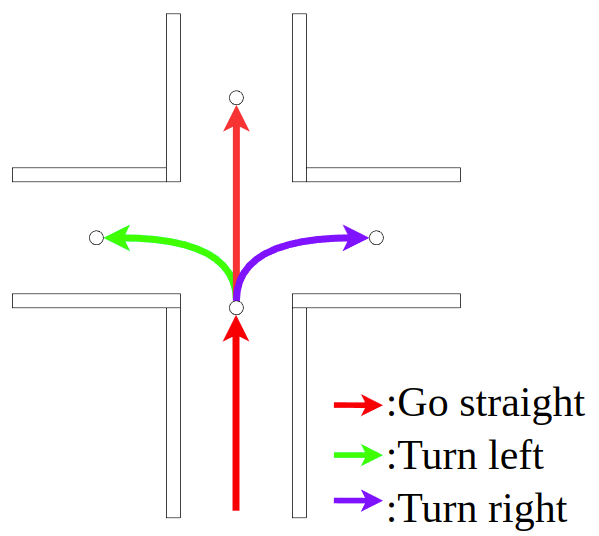
\includegraphics[keepaspectratio, scale=0.45]
      {images/direction.png}
 \caption{Target direction}
 \label{Fig:direction}
\end{figure}

学習器には, 上記の3つの目標方向を要素数3, 次元数1のint型の配列で表現した”目標方向指令”を入力する. 目標方向指令のデータ形式を\tabref{table:direction}に示す.

\begin{table}[hbtp]
  \caption{Target direction list}
  \label{table:direction}
  \centering
  \begin{tabular}{|c|c|c|c|}
    \hline
    Target Direction  & Go straight & Turn left & Trun right\\
    \hline
    Data & [100, 0, 0] & [0, 100, 0] & [0, 0, 100]\\
    \hline
  \end{tabular}
\end{table}

% \begin{figure}[hbtp]
%   \centering
%  \includegraphics[keepaspectratio, scale=0.45]
%       {images/direction.png}
%  \caption{Learning phase system of proposed method}
%  \label{Fig:direction}
% \end{figure}

% \subsubsection{etc...}
\newpage
